\section{结果评价}
\label{sec:rs-evaluation}

前面每种方法都给出了手算和几幅运行图。于是要问：两种随机搜索的结果怎样比才算数，一次运行结束时能下什么结论？要把三类说法分开：有限预算内得到了什么，长期运行有什么极限性质，以及能否验证结果确实接近最优。

\subsection{停止条件}
\label{sec:rs-eval-stop}

算法要在某一刻停下来。这一小节的问题是：各种停止规则分别支持什么结论？

\paragraph{四种规则}
\textbf{评价次数上限}在用完$B$次后停止，这是最容易比较的一种。\textbf{时间上限}在规定的墙钟时间后停止，它依赖机器和实现。\textbf{目标阈值}在$f_{\mathrm{best}}\leq f_{\mathrm{target}}$时停止，要有事先给定的阈值。\textbf{停滞规则}在连续若干轮没有改善时停止。

\paragraph{停滞规则只描述已观察到的过程}
图~\ref{fig:rs-eval-budget}(c)是五维Rastrigin问题上遗传算法的一次运行。最好值从第$300$次评价前后开始，在$10.28$上停了$500$多次评价，接着又下降，最后约为$0.02$。若规则是“连续$500$次评价没有改善就停”，这次运行就会在那段平台上结束，报告$10.28$。

停滞规则说的是最近没有发现更好的点，不代表不存在更好的点。它是预算的管理手段，不是最优性的判据。分布的$\sigma$变小、粒子聚集、种群趋同也都一样。

\paragraph{有下界时报告间隙}
能证明$\ell\leq f^\star$时，可行解$\hat{\bm{x}}$的目标差不超过$f(\hat{\bm{x}})-\ell$，这是可以验证的结论，第~\ref{chap:optimization}章讨论过这种夹逼。

第~\ref{sec:rs-ga}节的背包问题就是如此：把物品按价值密度排序，允许最后一件取一部分，得到的分数背包最优值是原问题价值的上界，也就是代价的下界。那里的六件物品按价值密度排序，取第$1,2,3$件用去重量$11$，再取第$4$件的$4/7$，分数解的总价值为$19+\tfrac47\times9\approx24.14$。价值都是整数，所以$f^\star\geq-24$，最好可行解$-23$与最优值至多差$1$，这是不依赖搜索过程的结论。

大多数黑箱问题没有可靠的下界。这时老实的报告是：最好可行值是多少，用了多少次评价。不能写“达到全局最优”，因为最优值未知，而$f(\hat{\bm{x}})-f^\star$根本无从计算。

\subsection{预算与重复运行}
\label{sec:rs-eval-budget}

停下来以后要比较。这一小节的问题是：不同算法的成本怎样折算到同一单位，一次运行不够时要比较什么？

\paragraph{统一的成本单位}
不同算法的“一轮”含义不同：退火的一轮是一次评价，CMA-ES的一代是$\lambda$次，粒子群的一轮是$N$次。按轮数比较没有意义，必须换算成实际的函数调用次数。表~\ref{tab:rs-cost-accounting}列出需要计入的内容。

\begin{BookInlineTable}
 \centering
 \caption{成本的记录。第一类按评价次数统一累计，第二类另行报告。}
 \label{tab:rs-cost-accounting}
 \begin{tabular}{ll}
  \toprule
  类别 & 项目 \\
  \midrule
  函数调用 & 种群评价、退火尝试、修复后的评价 \\
  & 重复读数、最好解复核、重启 \\
  & 温度标定等试探性评价 \\
  \midrule
  内部运算 & CMA-ES的矩阵分解、排序 \\
  存储 & 种群、协方差矩阵、记忆位置 \\
  并行 & 群体通信、同步等待的时间 \\
  \bottomrule
 \end{tabular}
\end{BookInlineTable}

评价便宜时，内部运算可能反而占主导，这时只数评价次数是不够的；评价昂贵时，内部运算可以忽略。两者都要记下，分别报告。

\paragraph{结果是一个分布}
这些算法是随机的，一次运行的结果只是一个样本。比较时要固定问题、固定初始条件的抽取规则和预算，做若干次独立运行，比较结果的分布，例如中位数和四分位数。用一次最好的运行代表一个方法，或者挑选种子，都没有意义。

\paragraph{比较实验}
图~\ref{fig:rs-eval-budget}比较五种做法。问题是五维Rastrigin函数，搜索区域为$[-5.12,5.12]^5$，统一预算$B=10000$，每种方法独立运行$41$次。表~\ref{tab:rs-eval-summary}给出结束时的结果，“达标”指最好值不超过$3$。

\begin{BookInlineFigure}
 \centering
 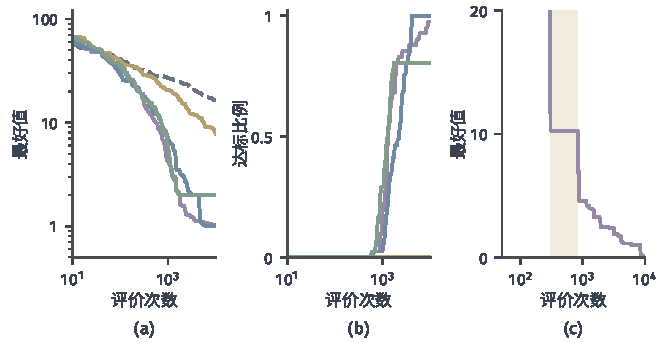
\includegraphics[width=112mm]{figures/05-optimization/05-stochastic-optimization/matplotlib/rs-eval-budget/figure.pdf}
 \caption{五维Rastrigin函数上的比较，$B=10000$，每种方法$41$次独立运行。灰色虚线为均匀随机抽样，黄线为模拟退火，紫线为实数编码遗传算法，蓝线为粒子群，绿线为CMA-ES。(a)最好值中位数随评价次数的变化。(b)最好值不超过$3$的运行所占比例。(c)遗传算法一次运行的最好值，浅黄区间是一段长约$530$次评价没有改善的平台。}
 \label{fig:rs-eval-budget}
\end{BookInlineFigure}

\begin{BookInlineTable}
 \centering
 \caption{$B=10000$时的结果（$41$次运行）。}
 \label{tab:rs-eval-summary}
 \begin{tabular}{lrrr}
  \toprule
  方法 & 中位数 & 上下四分位 & 达标比例 \\
  \midrule
  均匀随机抽样 & $16.49$ & $13.84$--$18.49$ & $0$ \\
  模拟退火 & $7.86$ & $5.69$--$10.35$ & $0$ \\
  遗传算法 & $1.03$ & $0.11$--$2.00$ & $0.98$ \\
  粒子群 & $0.99$ & $0.99$--$1.28$ & $1.00$ \\
  CMA-ES & $1.99$ & $0.99$--$2.98$ & $0.80$ \\
  \bottomrule
 \end{tabular}
\end{BookInlineTable}

这张表说明什么、不说明什么要说清楚。在这个问题、这组未专门调参的设置、这个预算下，三种基于群体或分布的方法达到了相近的量级，均匀抽样和这里的单点退火明显落后。

它不说明任何方法“更好”。退火换一组温度和提议尺度，结果可能大幅改变；CMA-ES此时已经收敛，后段的预算没有用上，加上重启可能改善；换一个问题，排序也可能颠倒。

图~\ref{fig:rs-eval-budget}(b)的曲线比一个终点数字更有信息：它回答了“要达到这个目标需要多少次评价”，三种方法都在约$10^3$次评价附近开始达标，CMA-ES的比例在约$0.8$处走平。

\paragraph{三类结论}
表~\ref{tab:rs-claims}把本章的结论按能够支持什么说法分类。写报告时，要清楚自己手里的结论属于哪一类。

\begin{BookInlineTable}
 \centering
 \caption{三类结论。}
 \label{tab:rs-claims}
 \begin{tabular}{ll}
  \toprule
  类别 & 例子与含义 \\
  \midrule
  有限预算的结果 & 中位数、达标比例：只对所测的设置成立 \\
  长期收敛结论 & 对数降温定理：是极限，并依赖模型条件 \\
  可验证的证书 & 下界与间隙：与算法如何运行无关 \\
  \bottomrule
 \end{tabular}
\end{BookInlineTable}
